% !TEX root = ../main.tex
\documentclass[../main.tex]{subfiles}

\begin{document}

\begin{figure}[h!]
    \centering
    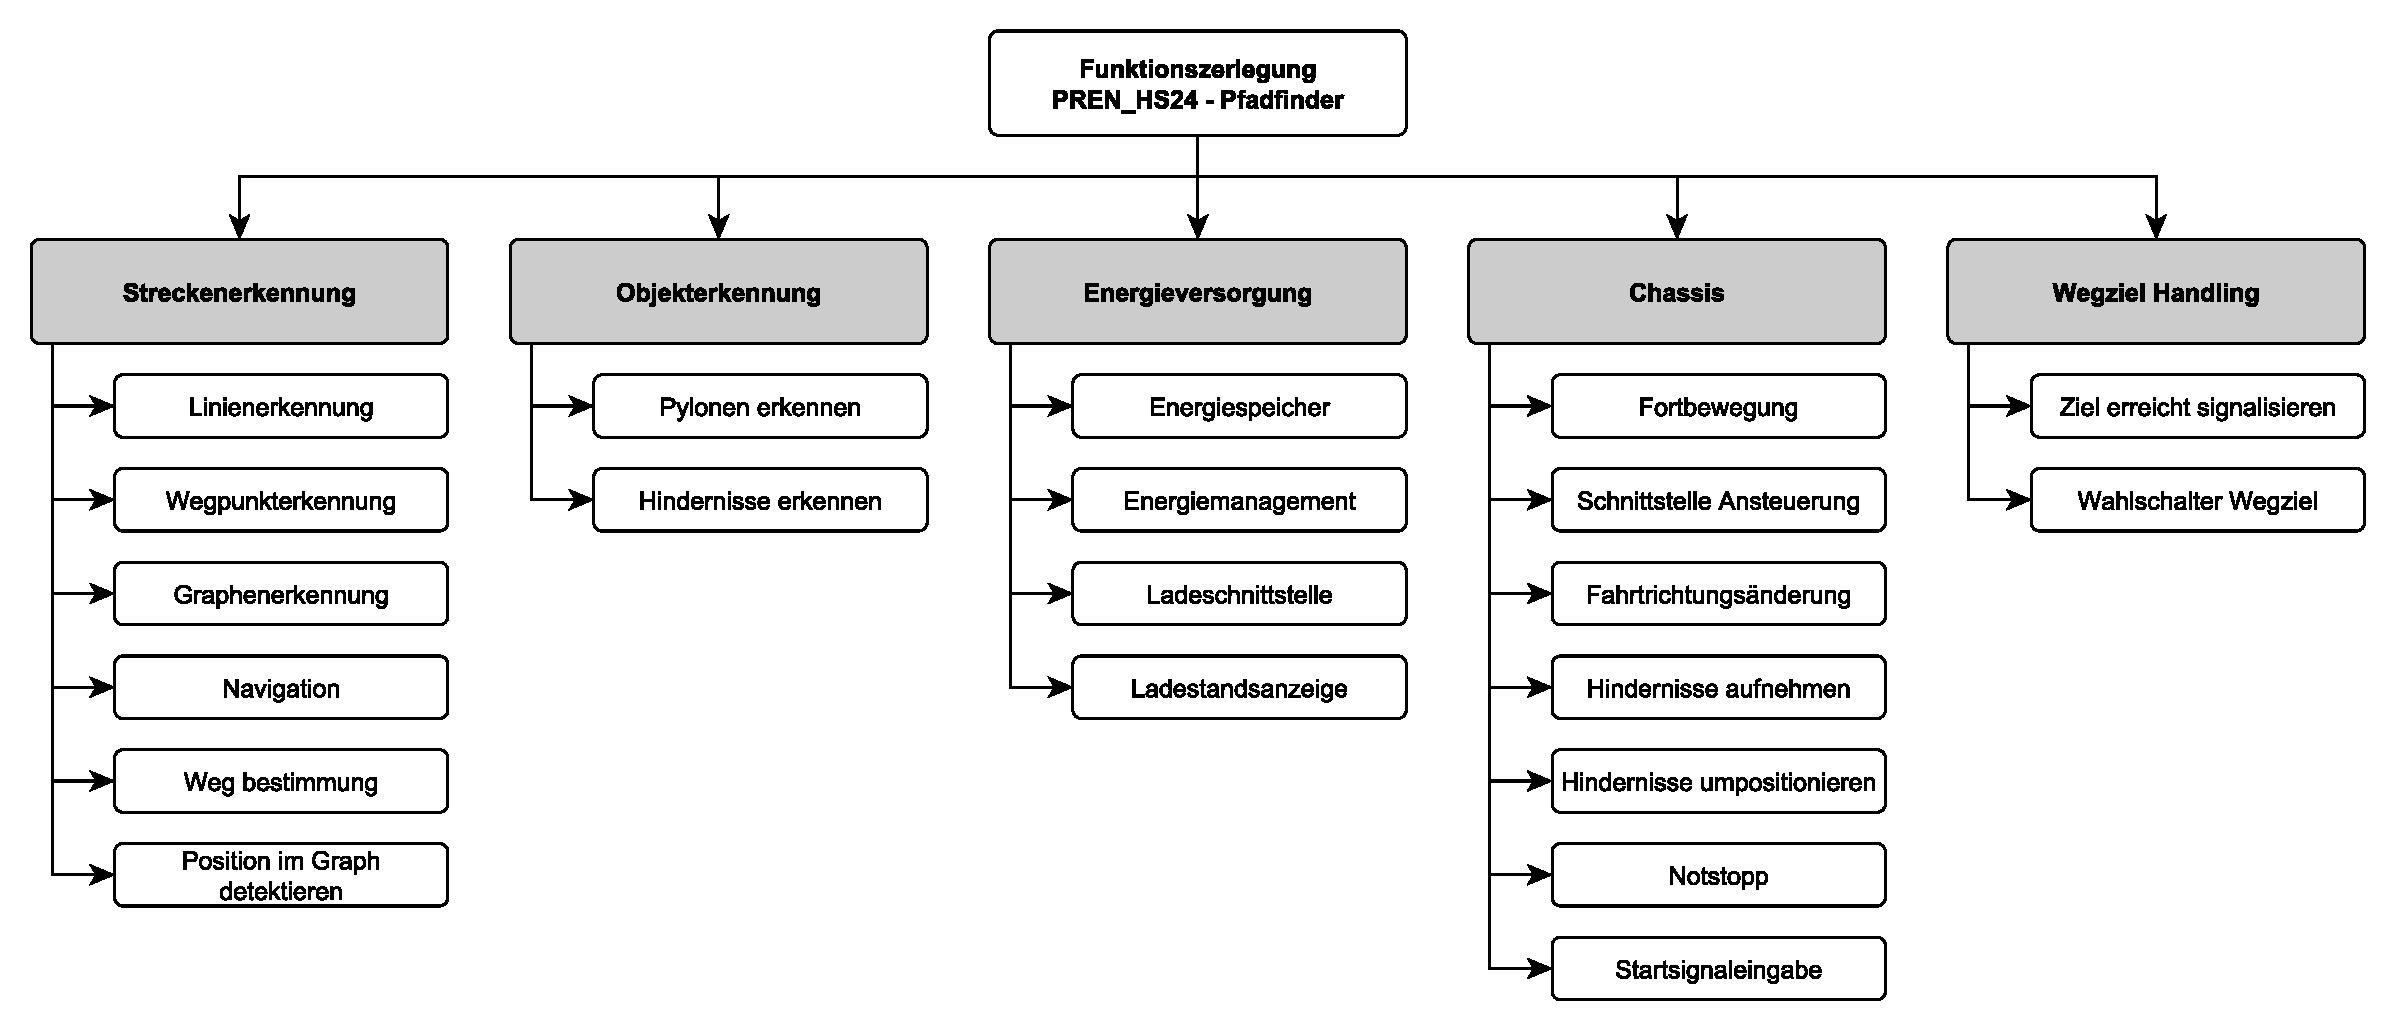
\includegraphics[width=1\textwidth]{./resources/Funktionszerlegung}
    \caption{Funktionszerlegung}\label{fig:Funktionszerlegung}
\end{figure}

Abbildung~\ref{fig:Funktionszerlegung} zeigt die Funktionszerlegung der
Hauptaufgabe des Pfadfinders, einen Weg durch das Wegenetz zu finden. Dabei ist
die Funktion auf einzelne notwendige Überkategorien aufgeteilt, zu welche
einzelne Unterfunktionen zugeordnet sind.

Kritische umzusetzende Funktionen stellen die Streckenerkennung und Navigation
dar. Von diesen Funktionen hängt die fehlerfreie Erfüllung der Aufgabe stark
ab.

\end{document}